\documentclass{dutmsc}%
%\documentclass[draft]{dutmsc}%
%
% STARTING FROM VERSION 1.0.8, DIRECT PDF OUTPUT FROM THE LATEX SOURCE IS SUPPORTED.
% IF YOU WANT TO USE THIS FEATURE, MAKE SURE ALL YOUR OWN FIGURES ARE IN A FORMAT
% SUPPORTED BY PDFLATEX, SO no EPS FILES, BUT PDF OR JPEG OR SO.
% THIS HAS CONSEQUENCES FOR THE PACKAGES USED AS WELL, pstricks CANNOT BE USED WITH PDFLATEX
%
% fill the following with relevant information
\mscDepartment{Aerodynamics and Wind Energy}%
\mscFaculty{Aerospace Engineering}%
\mscName{L. Manickathan B.Sc.}%
\mscDate{01.12.2013}%
\mscTitle{Hybrid Vortex Method for 2D Vertical-Axis Wind Turbine}%
\mscSubTitle{A fast and accurate Eulerian-Lagrangian numerical method in python}% can be left empty
\mscKeyWords{Hybrid Vortex Method, Python}%
%
% background picture for the first page, make sure it is in the correct format (eps or something else)
%\ifpdf
%  \mscBackPicture{./figs/merlin_landing_3_pdf}    % eps of 21 * 29.7 cm
%\else
%  \mscBackPicture{./figs/merlin_landing_3}    % pdf version of the cover background
%\fi
%
% readers page (un)comment as necessary
\mscReaderOne{prof.dr.ir. G.J.W. van Bussel}
\mscReaderTwo{dr.ir. C.J. Simao Ferreira}
\mscReaderThree{dr.ir. A. Palha da Silva Clerigo}
\mscReaderFour{prof.dr.ir. I. Bennett}
% \mscReaderFive{ir. Reader Five}
% \mscReaderSix{ir. Reader Six}
%
% if defined here with a non-zero (e.g. 1) argument, an entry will be added to 
% the table of contents for the list of figures and the list of tables,
% else they will not appear in the toc.
\loflotintoc{1}
%
% default install of latex on linux (tetex) does not include the apacite package, so using a local version
% if your latex distribution does provide it, you can uncomment the next two lines (and comment
% the two lines after that)
% \usepackage{apacite}%
% \bibliographystyle{apacite}%
% \usepackage{./local/apacite/apacite}%
%
% If you prefer references as numbers, comment the following line and uncomment the one thereafter
% \bibliographystyle{./local/apacite/apacite}%
\bibliographystyle{plain}
%
%
% use package breakurl to break url in sensible places (such as in www references)
% if it is not available in your latex distribution, use the local one
%\usepackage[preserveurlmacro]{./local/breakurl/breakurl}
\usepackage[preserveurlmacro]{breakurl}% %% Uncommented due to warning
%\usepackage{./local/breakurl/breakurl}%
%\usepackage{breakurl}% 
%
%=================%
% custom commands %
%=================%
%
% short-hand notations for cosine, sine and tangent with calligraphic C, S and T
\newcommand{\cc}[1]{\:\mathcal{C}_{#1}}%
\newcommand{\cs}[1]{\:\mathcal{S}_{#1}}%
\newcommand{\ct}[1]{\:\mathcal{T}_{#1}}%
%
% matlab in small caps
\newcommand{\matlab}{\textsc{Matlab} }
%
\makenomenclature
%
% setup of hyperlinks in the pdf output (modify as needed)
\hypersetup{colorlinks=true,
            citecolor=darkblue,
            urlcolor=darkred,
            linkcolor=darkblue,
            menucolor=darkblue,
            anchorcolor=red,
            pagecolor=cyan,
            pdfborder={0 0 0},
            bookmarksnumbered=true,
            breaklinks=true,
            pdfauthor={\mscname},           % value of \mscName
            pdftitle={\msctitle},           % value of \mscTitle
            pdfkeywords={\msckeywords}}     % value of \mscKeywords
%
\renewcommand{\bibname}{References}
\begin{document}%


%============================= Front matter ========================================
\frontmatter%
    %
    \maketitle%
    %
    % Abstract/summary
    \nonumchap{Summary}
    %
    This is the summary of the thesis.
%
    \cleardoublepage%
    %
    % thank people in this file
    \nonumchap{Acknowledgements}
    %
    
    The work I present here would not have been possible without the support of my supervisors dr.ir. C. (Carlos) J. Simao Ferreira and dr.ir. A. (Artur) Palha da Silva Clerigo. I want to thank Carlos for the constant encouragement and ensuring that I didn't loose myself in the detail and to have a global picture. Thank you for also giving me fresh perspective when it seems impossible and making me to think outside the box. I want to thank Artur for his daily supervision and guidance to teach me all the intricate details for developing this numerical method. I also want to thank him for putting aside time to work hand-in-hand to find solutions to the problems I faced and supporting me throughout the thesis.
    
    I want to thank my friends: Chid, Thor, Oliver, Mark, Rob, Alberto, Hector, Rody and Dieter for spending time together at the university, tackling the challenge of finishing the master thesis together. You guys gave me joy during the work and it was fun working beside you guys. I want to thank my friends: Nik, Vis, Adi, Srij, Ash, Vipul, Abi, Ram, Darsini, Yu, Ken, Gary, Hemmo and Dennis for making my last few years in Netherlands an enjoyable experience.
    
    Finally, I want to thank my family: Daddy, Mummy, Chechi, and Denis Chettan. Thank you for your patience and your unending love throughout my life.
    
    % signature containing place, name and date
    \signature
%
    \cleardoublepage%
    % 
    % table of contents, list of figures and list of tables
    \tocloflot%
    %
    % Nomenclature
    \printnomencl%
    \cleardoublepage%
    %
    %
\mainmatter%
    %
    % parts are not necessary for a thesis
    %
    % Example Chapter
    %\chapter{Introduction}
    %
    \section{Before You Start}
        %
        RTFM\footnote{Read The Fabulous Manual ;-)}: \href{http://www.ctan.org/tex-archive/info/lshort/english/lshort.pdf}{The Not So Short Introduction to \LaTeXe}.
        %
        Chapters 1, 2 and 3 are a must.
        
        And you directly see why \LaTeX~is so much easier than Word, external references actually work.
        %
        %
    \section{Quick Compilation of Your Thesis}
        %
        To quickly compile your thesis without processing all figures, add \verb+draft+ to the list of optional arguments of the main file (\verb+my_thesis.tex+ in this case):
        %
        \begin{verbatim}
    \documentclass[draft]{dutmsc}%
        \end{verbatim}
        %
        The actual figures will not appear, only a border will be shown. This reduces the compilation time by a significant amount. The command \verb+\includeonly{filelist}+ can also be used to only process the chapter you are working on at the time.
        %
    \section{Custom Commands}
        %
        \subsection{Vertical Spacing in Tables}
            %
            Look at Table~\ref{tab:sample_table}. Iz nice, no?
            %
            \begin{table}[!htb]
                \centering
                \begin{tabular}{ c c c }
                    \hline
                    Param\T\B                   & Value   & Unit    \\
                    \hline
                    $v_i$\T                     & 11.47   & $[m/s]$ \\
                    $\Omega R$                  & 212.25  & $[m/s]$ \\
                    $\lambda_i$\B               & 0.054   & $[-]$   \\
                    \hline
                \end{tabular}
                \caption{Improved vertical spacing in tables}\label{tab:sample_table}
            \end{table}
            %
            It uses two custom commands to add some space just after (bottom) and before (top) a horizontal line, \verb+\B+ and \verb+\T+. Without them, the table would look really bad (see Table~\ref{tab:sample_table2}).
            
            %
            \begin{table}[!htb]
                \centering
                \begin{tabular}{ c c c }
                    \hline
                    Param                       & Value   & Unit    \\
                    \hline
                    $v_i$                       & 11.47   & $[m/s]$ \\
                    $\Omega R$                  & 212.25  & $[m/s]$ \\
                    $\lambda_i$                 & 0.054   & $[-]$   \\
                    \hline
                \end{tabular}
                \caption{Default vertical spacing in tables}\label{tab:sample_table2}
            \end{table}
            %
        \subsection{Shorthand Notations for Sine, Cosine and Tangent}
            %
            Three commands are available to display sine, cosine and tangent of angles in math mode: $\cc{\alpha}$, $\cs{\beta}$, $\ct{\gamma}$.
            %
        %
    \section{Bibliography/References}%
        %
        These are some references just for the sake of it. If you want to know more about ground effect models, consult~\cite{xin_phd}.
        For an introduction into helicopter aerodynamics, read~\cite{leishman_book}. And a reference to LAPACK~\cite{lug}.
        If you need to know more about the display options for citations, read the documentation that is provided in its manual \url{./local/apacite/apacite.pdf}.
        
        This thesis uses a bib-file (named \verb+biblio.bib+), which contains a database of references. \LaTeX~collects those references that were referred to in the thesis, and store them in the \verb+*.aux+ files (for this chapter in \verb+chap_introduction.aux+). And as long a the program \verb+bibtex+ is not executed, \LaTeX~will complain about undefined citations and a missing \verb+.bbl+ file (in this case \verb+my_thesis.bbl+). To solve this, execute \verb+bibtex+. If everything goes as it should, a \verb+my_thesis.bbl+ is created, and the next time you run \LaTeX, a section with references will appear.
        
        Using \verb+Kile+ (on Linux), BibTex can be executed from the \verb+Build -> Compile -> Bibtex+ menu, or using the shortcut \verb/ALT+-/ (as in ALT+minus).
        
        Using \verb+TeXnicCenter+, BibTex can be executed from the \verb+Build -> BibTex+ or \\
        \verb+Build -> Current File -> BibTex+ menu.
        
        Using \verb+WinEdt+, BibTex can be executed with the shortcut \verb/CTL+SHIFT+B/ or from the menu \verb/Accessories -> BibTex/.
        %
    \section{Symbols and Units}%
        %
        For symbols, we use the \verb+nomencl+ package, of which you need the latest version (version 4.2, dated 2005/09/22).
        %
        \subsection{Summary of Commands}
            %
            For nomenclature (symbols and abbreviations) to appear in the nomenclature chapter, the following 6 categories are available:
            
            \begin{description}
                \item[Latin Symbols]    \verb+\lsymb[t]{symbol}{description}{unit}{sortsymbol}+
                \item[Greek Symbols]    \verb+\gsymb[t]{symbol}{description}{unit}{sortsymbol}+
                \item[Other Symbols]    \verb+\osymb[f]{symbol}{description}{sortsymbol}+
                \item[Superscripts]     \verb+\subscr[f]{symbol}{description}+
                \item[Subscripts]       \verb+\superscr[f]{symbol}{description}+
                \item[Abbreviations]    \verb+\acron[f]{abbreviation}{description}+
            \end{description}
            %
            The first option (with the square brackets) is an optional argument that lets you control the appearance of the symbol in the text at the place where the command appears. If it is equal to \emph{t}, the symbol will appear in the text and in the nomenclature list and otherwise, it will only appear in the nomenclature list. By default, Greek and Latin symbols will appear in the text, even if the optional symbol is not set. In case they should not appear, you have to add \verb|[f]| as first argument. In the above list, the default values are given, so by default, only the Greek and Latin symbols will appear in the text at the place where the commands appear.
            
            Now, if you want these symbols to appear in the \emph{Nomenclature list}, execute \verb+makeindex+\footnote{Note that makeindex is a program on your computer. It is not a \LaTeX~command!}:
            %
            \begin{small}
            \begin{verbatim}
   makeindex $THESIS_NAME.nlo -s nomencl.ist -o $THESIS_NAME.nls
            \end{verbatim}
            \end{small}
            %
            where \verb+$THESIS_NAME+ is the name of the main file (without extension), in this case \verb+my_thesis+. Depending on the editor you use, it may not be necessary to resort to command line magic, you might just have to press a button that defines a macro. Another solutions is to use the \emph{bat} file included in the same directory: \verb+sort_symb.bat+. Executing this should do the above automagically.
            
            %
            \subsubsection{Sorting Symbols}
                %
                To sort symbols properly, an additional fourth mandatory argument is added to the Greek, Latin and Other symbols. These add the ability to sort similar symbols (such as \lsymb[t]{$\dot{m}$}{mass flow}{$[kg/s]$}{mz} and \lsymb[t]{$m$}{mass}{$[kg]$}{mm}) in the proper order ($m$ before $\dot{m}$). The way to make sure that the symbol for mass flow appears after the symbol for mass is shown below:%
                %
                \begin{small}%
                \begin{verbatim}
    \lsymb[t]{$m$}{mass}{$[kg]$}{mm}
    \lsymb[t]{$\dot{m}$}{mass flow}{$[kg/s]$}{mz}
                \end{verbatim}%
                \end{small}%
                %
                \verb+mz+ comes after \verb+mm+ when sorted by \verb+makeindex+, which means that the symbol of mass flow will be put after the symbol for mass.
                
                Something similar can be done for the Greek symbols. If \gsymb[t]{$\gamma$}{flight path angle}{$[rad]$}{3} (third letter in the Greek alphabet) should appear before \gsymb[t]{$\delta$}{some coefficient to show proper sorting of symbols}{$[-]$}{4} (fourth letter), add a letter to force proper sorting:
                %
                \begin{small}%
                \begin{verbatim}
    \gsymb[t]{$\gamma$}{flight path angle}{$[rad]$}{cc}
    \gsymb[t]{$\delta$}{some coefficient to show proper sorting of symbols}{$[-]$}{4}
                \end{verbatim}%
                \end{small}%
                %
                In table~\ref{tab:greek_symbols}, you can find the sort symbols (index) that I used to make sure that the Greek symbols appear in the correct order in the nomenclature.
                %
                \begin{table}[!ht]
                    \centering
                    \begin{tabular}{c c c | c c c}
                        \hline
                        Greek Symbol\T\B  & Command     & Index & Greek Symbol\T\B  & Command     & Index \\
                        \hline
                        $\alpha$\T  & \verb+\alpha+     & aa    & $o$         & \verb+o+          & oo    \\
                        $\beta$     & \verb+\beta+      & bb    & $\Pi$       & \verb+\Pi+        & p     \\
                        $\Gamma$    & \verb+\Gamma+     & c     & $\pi$       & \verb+\pi+        & pp    \\
                        $\gamma$    & \verb+\gamma+     & cc    & $\rho$      & \verb+\rho+       & qq    \\
                        $\Delta$    & \verb+\Delta+     & d     & $\Sigma$    & \verb+\Sigma+     & r     \\
                        $\delta$    & \verb+\delta+     & dd    & $\sigma$    & \verb+\sigma+     & rr    \\
                        $\epsilon$  & \verb+\epsilon+   & ee    & $\tau$      & \verb+\tau+       & ss    \\
                        $\zeta$     & \verb+\zeta+      & ff    & $\Upsilon$  & \verb+\Upsilon+   & t     \\
                        $\eta$      & \verb+\eta+       & gg    & $\upsilon$  & \verb+\upsilon+   & tt    \\
                        $\Theta$    & \verb+\Theta+     & h     & $\Phi$      & \verb+\Phi+       & u     \\
                        $\theta$    & \verb+\theta+     & hh    & $\phi$      & \verb+\phi+       & uu    \\
                        $\iota$     & \verb+\iota+      & ii    & $\chi$      & \verb+\chi+       & vv    \\
                        $\kappa$    & \verb+\kappa+     & jj    & $\Psi$      & \verb+\Psi+       & w     \\
                        $\Lambda$   & \verb+\Lambda+    & k     & $\psi$      & \verb+\psi+       & ww    \\
                        $\lambda$   & \verb+\lambda+    & kk    & $\omega$    & \verb+\omega+     & xx    \\
                        $\mu$       & \verb+\mu+        & ll    & $\Omega$\B  & \verb+\Omega+     & x     \\
                        $\nu$       & \verb+\nu+        & mm    &  &  & \\
                        $\Xi$       & \verb+\Xi+        & n     &  &  & \\
                        $\xi$       & \verb+\xi+        & nn    &  &  & \\
                        \hline
                    \end{tabular}
                    \caption{Sort symbols used to sort all Greek letters}\label{tab:greek_symbols}
                \end{table}
                %
        \subsection{More Examples}
            %
            The angle of attack \gsymb[f]{$\alpha$}{This is a very long explanation, and without this, it is still too short to show you what I want to show\ldots}{$[rad]$}{aa} (\verb+\gsymb[f]{\alpha}{Angle of attack}{$[rad]$}{aa}+) can be calculated from the pitch angle \gsymb{$\theta$}{Angle of pitch}{$[rad]$}{hh} (\verb+\gsymb{\theta}{Angle of pitch}{$[rad]$}{hh}+) and the flight path angle \gsymb{$\phi$}{Flight path angle}{$[rad]$}{uu} (\verb+\gsymb{\phi}{Flight path angle}{$[rad]$}{uu}+) as follows:
            %
            \begin{equation}
                \alpha = \theta + \phi\footnote{Note that the sign depends on the definition of the angles.}
            \end{equation}
            %
            Same thing for Latin symbols:
            
            \lsymb[t]{$\bar{x}$}{State vector of a dynamical system}{$[-]$}{xb}, for which the code looks like this:
            %
    \begin{verbatim}
    \lsymb[t]{$\bar{x}$}{State vector of a dynamical system}{$[-]$}{xb}
    \end{verbatim}
            %
            
            \begin{equation}\label{eq:state_vector_squared}
                \bar{x}^2 = \theta_i
            \end{equation}
            %
            \superscr[f]{2}{Square me}\subscr{i}{An index, or something\ldots}
            For subscripts and superscripts (as depicted in Eq~\ref{eq:state_vector_squared}), something special is needed. The sub- and superscripts must be added separately, as in:
            %
            \begin{verbatim}
    \superscr[f]{2}{Square me}\subscr{i}{An index, or something\ldots}
            \end{verbatim}
            %
            The commands for sub- and superscripts also have only two obligatory arguments, instead of three as is the case with the Latin and Greek symbols.
            
            Acronyms are also part of the nomenclature list. They are defined as follows:
            %
            \begin{verbatim}
    \acron[t]{PID}{Proportional -- Integral -- Derivative}
            \end{verbatim}
            %
            \acron[t]{P}{Proportional (Controller)}, 
            \acron[t]{PD}{Proportional -- Derivative (Controller)} and
            \acron[t]{PID}{Proportional -- Integral -- Derivative (Controller)} controllers.
            
            At last, there is a possibility for other symbols that do not fit in any of the above categories, such as symbols to denote matrices or vector quantities, such as \osymb[t]{$[\;]$}{matrix}, \osymb[t]{$\{\;\}$}{column vector} and \osymb[t]{$\bar{\;}$}{vector quantity}.
            %
    \section{Figures}
        %
        Up to version 1.0.7 of the style file, the only option to generate pdf output was throught the three-step process LATEX $\rightarrow$ DVI, DVI $\rightarrow$ PS, PS $\rightarrow$ PDF.
        
        Starting from version 1.0.8, direct pdf output is supported as well. This has some consequences for the file formats of figuress that are supported. When creating the pdf directly, figures in (encapsulated) postscript format will give errors. Convert them to pdf format.
        
        In all previous versions of this document, the advice in this section was to save all plots and figures as PostScript, and not as PDF. Processing your \LaTeX~input using LATEX $\rightarrow$ DVI, DVI $\rightarrow$ PS, PS $\rightarrow$ PDF works without problems. An added benefit is that you can use the \emph{psfrag} package to replace ordinary text characters in the postscript figures by e.g. mathematical formulas typeset in \LaTeX. Also, one can use the \emph{pstricks} packages to create figures (see~\href{http://www.tug.org/PSTricks/main.cgi/}{PSTricks packages}) directly in \LaTeX.
        
        The same can be achieved with plot output from e.g. {\sc matlab} using \emph{LaPrint}.
        
        LaPrint is a {\sc matlab} function to print {\sc matlab} graphics for inclusion in \LaTeX~documents. LaPrint creates an eps-file and a tex-file. The tex-file contains the annotation of the figure such as titles, labels and texts. The eps-file contains the non-text part of the figure and is called by the tex-file. 
        
        The main advantage of using LaPrint is that the annotation can be neatly (e.g., including math mode and fancy font constructs) set within \LaTeX. LaPrint can be used from the command line or via a graphical user interface (GUI).
        
        A Users Guide for LaPrint is available at \href{http://www.uni-kassel.de/fb16/rat/matlab/laprint/laprintdoc.ps}{\burl{http://www.uni-kassel.de/fb16/rat/matlab/laprint/laprintdoc.ps}}.
        The m-file can be downloaded from \href{http://www.mathworks.de/matlabcentral/fileexchange/4638}{Matlab File Exchange}.
        

        
%         {\LARGE For the best results and the least amount of headaches, save all your plots and figures as {\Huge PostScript}, not as PDF.}
%         
%         And process your \LaTeX~input using: LATEX $\rightarrow$ DVI, DVI $\rightarrow$ PS, PS $\rightarrow$ PDF. That way, you can use the \emph{psfrag} package to replace characters in a postscript file with formulas in the correct font, as will be shown below. Figure~\ref{fig:sideview_reference_frames} is the original, produced with XFig and saved as an Encapsulated PostScript file.
        \subsection{Some Examples}%
%         In Figure~\ref{fig:sideview_reference_frames_2}, the same figure is used, only here, all strings are replaced with properly typeset \emph{formulas}.
        %
        \begin{figure}[!hbt]
            \centering
            \ifpdf
              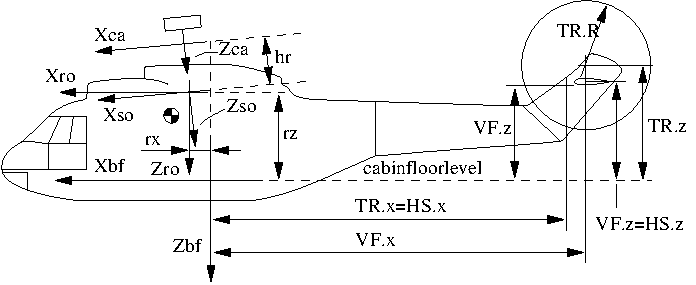
\includegraphics[width=0.7\textwidth]{./figs/chap_introduction/heli_sideview_pdf}
            \else
              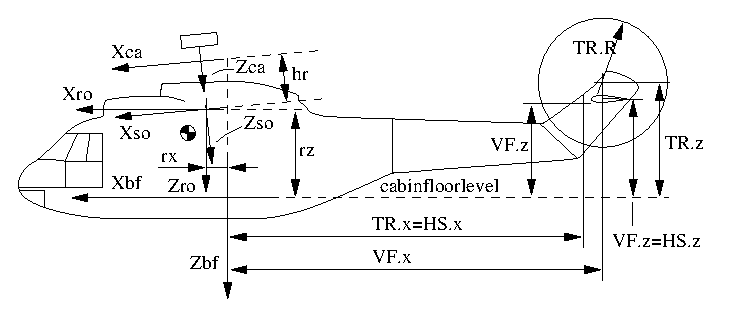
\includegraphics[width=0.7\textwidth]{./figs/chap_introduction/heli_sideview}
            \fi
            \caption[Short caption in the lof: schematic sideview of a helicopter]{Schematic sideview of a helicopter that is by now most likely too long to fit on one line.}
            \label{fig:sideview_reference_frames}
        \end{figure}
        %
%        \begin{figure}[!hbt]
%%             \tiny
%%             \scriptsize
%            \footnotesize
%            \psfrag{Xca}{$\mathsf{X_{hp}}$}
%            \psfrag{Zca}{$\mathsf{Z_{hp}}$}
%            \psfrag{Xro}{$\mathsf{X_{ro}}$}
%            \psfrag{Zro}{$\mathsf{Z_{ro}}$}
%            \psfrag{Xso}{$\mathsf{X_{so}}$}
%            \psfrag{Zso}{$\mathsf{Z_{so}}$}
%            \psfrag{Xbf}{$\mathsf{X_{bf}}$}
%            \psfrag{Zbf}{$\mathsf{Z_{bf}}$}
%            \psfrag{cabinfloorlevel}{$\mathsf{cabin floorlevel}$}
%            \psfrag{TR.R}{$\mathsf{R_{tr}}$}
%            \psfrag{TR.z}{$\mathsf{z_{tr}}$}
%            \psfrag{TR.x=HS.x}{$\mathsf{x_{vf}}$}
%            \psfrag{HS.z}{$\mathsf{z_{hs}}$}
%            \psfrag{VF.z=HS.z}{$\mathsf{z_{hs}}$}
%            \psfrag{VF.z}{$z_{vf}$}
%            \psfrag{VF.x}{$x_{tr} = x_{hs}$}
%            \psfrag{hr}{$h_{r}$}
%            \psfrag{rx}{$r_{x}$}
%            \psfrag{rz}{$r_{z}$}
%            \centering
%            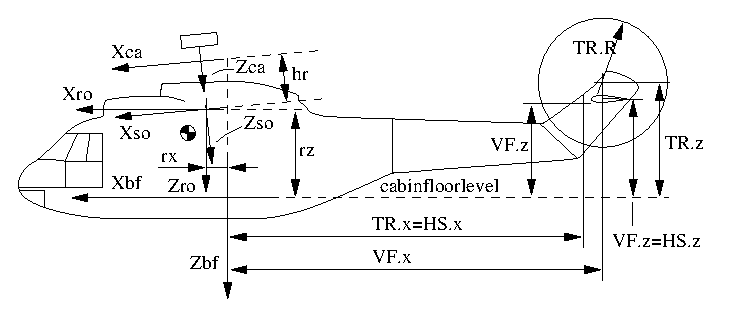
\includegraphics[width=0.7\textwidth]{./figs/chap_introduction/heli_sideview}
%            \caption{Schematic sideview of a helicopter (2)}
%            \label{fig:sideview_reference_frames_2}
%        \end{figure}
        %
        And a fancy figure to show you what is possible with graphics in \LaTeX, see Figure~\ref{fig:blade_geometry}.
        %
%        \begin{figure}[!htb]
%            \centering
%            \subfloat[Equal annuli segment distribution]{%
%                \begin{pspicture}(-0.25,-0.25)(13.125,1.2)
%                    % \psgrid[subgriddiv=1,griddots=10,gridlabels=7pt]
%                    \psdot*[dotsize=4pt](0,0)
%                    % quarter chord line
%                    \psline{-}(-0.25,0)(13.125,0)
%                    % vertical line through centre of rotation
%                    \psline{-}(0,-0.25)(0,0.25)
%                    % blade contours
%                    \pspolygon(3.0625,-0.2363)(13.125,-0.2363)(13.125,0.7088)(3.0625,0.7088)
%                    % blade segment sides
%                    \psline(5.0663,  -0.2363)( 5.0663,  0.7088)
%                    \psline(6.4775,  -0.2363)( 6.4775,  0.7088)
%                    \psline(7.6318,  -0.2363)( 7.6318,  0.7088)
%                    \psline(8.6333,  -0.2363)( 8.6333,  0.7088)
%                    \psline(9.5302,  -0.2363)( 9.5302,  0.7088)
%                    \psline(10.3495, -0.2363)( 10.3495, 0.7088)
%                    \psline(11.1085, -0.2363)( 11.1085, 0.7088)
%                    \psline(11.8190, -0.2363)( 11.8190, 0.7088)
%                    \psline(12.4891, -0.2363)( 12.4891, 0.7088)
%                    % control points
%                    \psdots*[dotsize=4pt](4.0644,  0.0)(5.7719,  0.0)(7.0546,  0.0)(8.1325,  0.0)(9.0817,  0.0)(9.9398,  0.0)(10.7290, 0.0)(11.4637, 0.0)(12.1540, 0.0)(12.8070, 0.0)
%                \end{pspicture}\label{subfig:equal_anulli_distribution}}\\
%            \subfloat[Constant width segment distribution]{%
%                \begin{pspicture}(-0.25,-0.25)(13.125,1.2)
%                    % \psgrid[subgriddiv=1,griddots=10,gridlabels=7pt]
%                    \psdot*[dotsize=4pt](0,0)
%                    % quarter chord line
%                    \psline{-}(-0.25,0)(13.125,0)
%                    % vertical line through centre of rotation
%                    \psline{-}(0,-0.25)(0,0.25)
%                    % blade contours
%                    \pspolygon(3.0625,-0.2363)(13.125,-0.2363)(13.125,0.7088)(3.0625,0.7088)
%                    % blade segment sides
%                    \psline(3.0625,  -0.2363)( 3.0625,  0.7088)
%                    \psline(4.0688,  -0.2363)( 4.0688,  0.7088)
%                    \psline(5.0750,  -0.2363)( 5.0750,  0.7088)
%                    \psline(6.0813,  -0.2363)( 6.0813,  0.7088)
%                    \psline(7.0875,  -0.2363)( 7.0875,  0.7088)
%                    \psline(8.0938,  -0.2363)( 8.0938, 0.7088)
%                    \psline(9.1000,  -0.2363)( 9.1000,  0.7088)
%                    \psline(10.1063, -0.2363)( 10.1063, 0.7088)
%                    \psline(11.1125, -0.2363)( 11.1125, 0.7088)
%                    \psline(12.1188, -0.2363)( 12.1188, 0.7088)
%                    \psline(13.1250, -0.2363)( 13.1250, 0.7088)
%                    % control points
%                    \psdots*[dotsize=4pt](3.5656,  0.00)(4.5719,  0.00)(5.5781,  0.00)(6.5844,  0.00)(7.5906,  0.00)(8.5969,  0.00)(9.6031,  0.00)(10.6094, 0.00)(11.6156, 0.00)(12.6219, 0.00)
%                \end{pspicture}\label{subfig:constant_width_distribution}}
%            \caption[Geometry for a helicopter main rotor blade]{Geometry and segment distributions for a helicopter main rotor blade with 10 segments} \label{fig:blade_geometry}
%        \end{figure}
        %
    \subsection{Alternatives}%
        %
        An alternative to saving figures as PostScript is saving them as PDF. Then, you have to use \emph{pdflatex} which skips the intermediate files. Please note that I will not provide support if you run into problems when you decide to do it this way.
        
        
    % Chapter 1: Introduction
    \chapter{Introduction}
    %
    \section{Before You Start}
        %
        RTFM\footnote{Read The Fabulous Manual ;-)}: \href{http://www.ctan.org/tex-archive/info/lshort/english/lshort.pdf}{The Not So Short Introduction to \LaTeXe}.
        %
        Chapters 1, 2 and 3 are a must.
        
        And you directly see why \LaTeX~is so much easier than Word, external references actually work.
        %
        %
    \section{Quick Compilation of Your Thesis}
        %
        To quickly compile your thesis without processing all figures, add \verb+draft+ to the list of optional arguments of the main file (\verb+my_thesis.tex+ in this case):
        %
        \begin{verbatim}
    \documentclass[draft]{dutmsc}%
        \end{verbatim}
        %
        The actual figures will not appear, only a border will be shown. This reduces the compilation time by a significant amount. The command \verb+\includeonly{filelist}+ can also be used to only process the chapter you are working on at the time.
        %
    \section{Custom Commands}
        %
        \subsection{Vertical Spacing in Tables}
            %
            Look at Table~\ref{tab:sample_table}. Iz nice, no?
            %
            \begin{table}[!htb]
                \centering
                \begin{tabular}{ c c c }
                    \hline
                    Param\T\B                   & Value   & Unit    \\
                    \hline
                    $v_i$\T                     & 11.47   & $[m/s]$ \\
                    $\Omega R$                  & 212.25  & $[m/s]$ \\
                    $\lambda_i$\B               & 0.054   & $[-]$   \\
                    \hline
                \end{tabular}
                \caption{Improved vertical spacing in tables}\label{tab:sample_table}
            \end{table}
            %
            It uses two custom commands to add some space just after (bottom) and before (top) a horizontal line, \verb+\B+ and \verb+\T+. Without them, the table would look really bad (see Table~\ref{tab:sample_table2}).
            
            %
            \begin{table}[!htb]
                \centering
                \begin{tabular}{ c c c }
                    \hline
                    Param                       & Value   & Unit    \\
                    \hline
                    $v_i$                       & 11.47   & $[m/s]$ \\
                    $\Omega R$                  & 212.25  & $[m/s]$ \\
                    $\lambda_i$                 & 0.054   & $[-]$   \\
                    \hline
                \end{tabular}
                \caption{Default vertical spacing in tables}\label{tab:sample_table2}
            \end{table}
            %
        \subsection{Shorthand Notations for Sine, Cosine and Tangent}
            %
            Three commands are available to display sine, cosine and tangent of angles in math mode: $\cc{\alpha}$, $\cs{\beta}$, $\ct{\gamma}$.
            %
        %
    \section{Bibliography/References}%
        %
        These are some references just for the sake of it. If you want to know more about ground effect models, consult~\cite{xin_phd}.
        For an introduction into helicopter aerodynamics, read~\cite{leishman_book}. And a reference to LAPACK~\cite{lug}.
        If you need to know more about the display options for citations, read the documentation that is provided in its manual \url{./local/apacite/apacite.pdf}.
        
        This thesis uses a bib-file (named \verb+biblio.bib+), which contains a database of references. \LaTeX~collects those references that were referred to in the thesis, and store them in the \verb+*.aux+ files (for this chapter in \verb+chap_introduction.aux+). And as long a the program \verb+bibtex+ is not executed, \LaTeX~will complain about undefined citations and a missing \verb+.bbl+ file (in this case \verb+my_thesis.bbl+). To solve this, execute \verb+bibtex+. If everything goes as it should, a \verb+my_thesis.bbl+ is created, and the next time you run \LaTeX, a section with references will appear.
        
        Using \verb+Kile+ (on Linux), BibTex can be executed from the \verb+Build -> Compile -> Bibtex+ menu, or using the shortcut \verb/ALT+-/ (as in ALT+minus).
        
        Using \verb+TeXnicCenter+, BibTex can be executed from the \verb+Build -> BibTex+ or \\
        \verb+Build -> Current File -> BibTex+ menu.
        
        Using \verb+WinEdt+, BibTex can be executed with the shortcut \verb/CTL+SHIFT+B/ or from the menu \verb/Accessories -> BibTex/.
        %
    \section{Symbols and Units}%
        %
        For symbols, we use the \verb+nomencl+ package, of which you need the latest version (version 4.2, dated 2005/09/22).
        %
        \subsection{Summary of Commands}
            %
            For nomenclature (symbols and abbreviations) to appear in the nomenclature chapter, the following 6 categories are available:
            
            \begin{description}
                \item[Latin Symbols]    \verb+\lsymb[t]{symbol}{description}{unit}{sortsymbol}+
                \item[Greek Symbols]    \verb+\gsymb[t]{symbol}{description}{unit}{sortsymbol}+
                \item[Other Symbols]    \verb+\osymb[f]{symbol}{description}{sortsymbol}+
                \item[Superscripts]     \verb+\subscr[f]{symbol}{description}+
                \item[Subscripts]       \verb+\superscr[f]{symbol}{description}+
                \item[Abbreviations]    \verb+\acron[f]{abbreviation}{description}+
            \end{description}
            %
            The first option (with the square brackets) is an optional argument that lets you control the appearance of the symbol in the text at the place where the command appears. If it is equal to \emph{t}, the symbol will appear in the text and in the nomenclature list and otherwise, it will only appear in the nomenclature list. By default, Greek and Latin symbols will appear in the text, even if the optional symbol is not set. In case they should not appear, you have to add \verb|[f]| as first argument. In the above list, the default values are given, so by default, only the Greek and Latin symbols will appear in the text at the place where the commands appear.
            
            Now, if you want these symbols to appear in the \emph{Nomenclature list}, execute \verb+makeindex+\footnote{Note that makeindex is a program on your computer. It is not a \LaTeX~command!}:
            %
            \begin{small}
            \begin{verbatim}
   makeindex $THESIS_NAME.nlo -s nomencl.ist -o $THESIS_NAME.nls
            \end{verbatim}
            \end{small}
            %
            where \verb+$THESIS_NAME+ is the name of the main file (without extension), in this case \verb+my_thesis+. Depending on the editor you use, it may not be necessary to resort to command line magic, you might just have to press a button that defines a macro. Another solutions is to use the \emph{bat} file included in the same directory: \verb+sort_symb.bat+. Executing this should do the above automagically.
            
            %
            \subsubsection{Sorting Symbols}
                %
                To sort symbols properly, an additional fourth mandatory argument is added to the Greek, Latin and Other symbols. These add the ability to sort similar symbols (such as \lsymb[t]{$\dot{m}$}{mass flow}{$[kg/s]$}{mz} and \lsymb[t]{$m$}{mass}{$[kg]$}{mm}) in the proper order ($m$ before $\dot{m}$). The way to make sure that the symbol for mass flow appears after the symbol for mass is shown below:%
                %
                \begin{small}%
                \begin{verbatim}
    \lsymb[t]{$m$}{mass}{$[kg]$}{mm}
    \lsymb[t]{$\dot{m}$}{mass flow}{$[kg/s]$}{mz}
                \end{verbatim}%
                \end{small}%
                %
                \verb+mz+ comes after \verb+mm+ when sorted by \verb+makeindex+, which means that the symbol of mass flow will be put after the symbol for mass.
                
                Something similar can be done for the Greek symbols. If \gsymb[t]{$\gamma$}{flight path angle}{$[rad]$}{3} (third letter in the Greek alphabet) should appear before \gsymb[t]{$\delta$}{some coefficient to show proper sorting of symbols}{$[-]$}{4} (fourth letter), add a letter to force proper sorting:
                %
                \begin{small}%
                \begin{verbatim}
    \gsymb[t]{$\gamma$}{flight path angle}{$[rad]$}{cc}
    \gsymb[t]{$\delta$}{some coefficient to show proper sorting of symbols}{$[-]$}{4}
                \end{verbatim}%
                \end{small}%
                %
                In table~\ref{tab:greek_symbols}, you can find the sort symbols (index) that I used to make sure that the Greek symbols appear in the correct order in the nomenclature.
                %
                \begin{table}[!ht]
                    \centering
                    \begin{tabular}{c c c | c c c}
                        \hline
                        Greek Symbol\T\B  & Command     & Index & Greek Symbol\T\B  & Command     & Index \\
                        \hline
                        $\alpha$\T  & \verb+\alpha+     & aa    & $o$         & \verb+o+          & oo    \\
                        $\beta$     & \verb+\beta+      & bb    & $\Pi$       & \verb+\Pi+        & p     \\
                        $\Gamma$    & \verb+\Gamma+     & c     & $\pi$       & \verb+\pi+        & pp    \\
                        $\gamma$    & \verb+\gamma+     & cc    & $\rho$      & \verb+\rho+       & qq    \\
                        $\Delta$    & \verb+\Delta+     & d     & $\Sigma$    & \verb+\Sigma+     & r     \\
                        $\delta$    & \verb+\delta+     & dd    & $\sigma$    & \verb+\sigma+     & rr    \\
                        $\epsilon$  & \verb+\epsilon+   & ee    & $\tau$      & \verb+\tau+       & ss    \\
                        $\zeta$     & \verb+\zeta+      & ff    & $\Upsilon$  & \verb+\Upsilon+   & t     \\
                        $\eta$      & \verb+\eta+       & gg    & $\upsilon$  & \verb+\upsilon+   & tt    \\
                        $\Theta$    & \verb+\Theta+     & h     & $\Phi$      & \verb+\Phi+       & u     \\
                        $\theta$    & \verb+\theta+     & hh    & $\phi$      & \verb+\phi+       & uu    \\
                        $\iota$     & \verb+\iota+      & ii    & $\chi$      & \verb+\chi+       & vv    \\
                        $\kappa$    & \verb+\kappa+     & jj    & $\Psi$      & \verb+\Psi+       & w     \\
                        $\Lambda$   & \verb+\Lambda+    & k     & $\psi$      & \verb+\psi+       & ww    \\
                        $\lambda$   & \verb+\lambda+    & kk    & $\omega$    & \verb+\omega+     & xx    \\
                        $\mu$       & \verb+\mu+        & ll    & $\Omega$\B  & \verb+\Omega+     & x     \\
                        $\nu$       & \verb+\nu+        & mm    &  &  & \\
                        $\Xi$       & \verb+\Xi+        & n     &  &  & \\
                        $\xi$       & \verb+\xi+        & nn    &  &  & \\
                        \hline
                    \end{tabular}
                    \caption{Sort symbols used to sort all Greek letters}\label{tab:greek_symbols}
                \end{table}
                %
        \subsection{More Examples}
            %
            The angle of attack \gsymb[f]{$\alpha$}{This is a very long explanation, and without this, it is still too short to show you what I want to show\ldots}{$[rad]$}{aa} (\verb+\gsymb[f]{\alpha}{Angle of attack}{$[rad]$}{aa}+) can be calculated from the pitch angle \gsymb{$\theta$}{Angle of pitch}{$[rad]$}{hh} (\verb+\gsymb{\theta}{Angle of pitch}{$[rad]$}{hh}+) and the flight path angle \gsymb{$\phi$}{Flight path angle}{$[rad]$}{uu} (\verb+\gsymb{\phi}{Flight path angle}{$[rad]$}{uu}+) as follows:
            %
            \begin{equation}
                \alpha = \theta + \phi\footnote{Note that the sign depends on the definition of the angles.}
            \end{equation}
            %
            Same thing for Latin symbols:
            
            \lsymb[t]{$\bar{x}$}{State vector of a dynamical system}{$[-]$}{xb}, for which the code looks like this:
            %
    \begin{verbatim}
    \lsymb[t]{$\bar{x}$}{State vector of a dynamical system}{$[-]$}{xb}
    \end{verbatim}
            %
            
            \begin{equation}\label{eq:state_vector_squared}
                \bar{x}^2 = \theta_i
            \end{equation}
            %
            \superscr[f]{2}{Square me}\subscr{i}{An index, or something\ldots}
            For subscripts and superscripts (as depicted in Eq~\ref{eq:state_vector_squared}), something special is needed. The sub- and superscripts must be added separately, as in:
            %
            \begin{verbatim}
    \superscr[f]{2}{Square me}\subscr{i}{An index, or something\ldots}
            \end{verbatim}
            %
            The commands for sub- and superscripts also have only two obligatory arguments, instead of three as is the case with the Latin and Greek symbols.
            
            Acronyms are also part of the nomenclature list. They are defined as follows:
            %
            \begin{verbatim}
    \acron[t]{PID}{Proportional -- Integral -- Derivative}
            \end{verbatim}
            %
            \acron[t]{P}{Proportional (Controller)}, 
            \acron[t]{PD}{Proportional -- Derivative (Controller)} and
            \acron[t]{PID}{Proportional -- Integral -- Derivative (Controller)} controllers.
            
            At last, there is a possibility for other symbols that do not fit in any of the above categories, such as symbols to denote matrices or vector quantities, such as \osymb[t]{$[\;]$}{matrix}, \osymb[t]{$\{\;\}$}{column vector} and \osymb[t]{$\bar{\;}$}{vector quantity}.
            %
    \section{Figures}
        %
        Up to version 1.0.7 of the style file, the only option to generate pdf output was throught the three-step process LATEX $\rightarrow$ DVI, DVI $\rightarrow$ PS, PS $\rightarrow$ PDF.
        
        Starting from version 1.0.8, direct pdf output is supported as well. This has some consequences for the file formats of figuress that are supported. When creating the pdf directly, figures in (encapsulated) postscript format will give errors. Convert them to pdf format.
        
        In all previous versions of this document, the advice in this section was to save all plots and figures as PostScript, and not as PDF. Processing your \LaTeX~input using LATEX $\rightarrow$ DVI, DVI $\rightarrow$ PS, PS $\rightarrow$ PDF works without problems. An added benefit is that you can use the \emph{psfrag} package to replace ordinary text characters in the postscript figures by e.g. mathematical formulas typeset in \LaTeX. Also, one can use the \emph{pstricks} packages to create figures (see~\href{http://www.tug.org/PSTricks/main.cgi/}{PSTricks packages}) directly in \LaTeX.
        
        The same can be achieved with plot output from e.g. {\sc matlab} using \emph{LaPrint}.
        
        LaPrint is a {\sc matlab} function to print {\sc matlab} graphics for inclusion in \LaTeX~documents. LaPrint creates an eps-file and a tex-file. The tex-file contains the annotation of the figure such as titles, labels and texts. The eps-file contains the non-text part of the figure and is called by the tex-file. 
        
        The main advantage of using LaPrint is that the annotation can be neatly (e.g., including math mode and fancy font constructs) set within \LaTeX. LaPrint can be used from the command line or via a graphical user interface (GUI).
        
        A Users Guide for LaPrint is available at \href{http://www.uni-kassel.de/fb16/rat/matlab/laprint/laprintdoc.ps}{\burl{http://www.uni-kassel.de/fb16/rat/matlab/laprint/laprintdoc.ps}}.
        The m-file can be downloaded from \href{http://www.mathworks.de/matlabcentral/fileexchange/4638}{Matlab File Exchange}.
        

        
%         {\LARGE For the best results and the least amount of headaches, save all your plots and figures as {\Huge PostScript}, not as PDF.}
%         
%         And process your \LaTeX~input using: LATEX $\rightarrow$ DVI, DVI $\rightarrow$ PS, PS $\rightarrow$ PDF. That way, you can use the \emph{psfrag} package to replace characters in a postscript file with formulas in the correct font, as will be shown below. Figure~\ref{fig:sideview_reference_frames} is the original, produced with XFig and saved as an Encapsulated PostScript file.
        \subsection{Some Examples}%
%         In Figure~\ref{fig:sideview_reference_frames_2}, the same figure is used, only here, all strings are replaced with properly typeset \emph{formulas}.
        %
        \begin{figure}[!hbt]
            \centering
            \ifpdf
              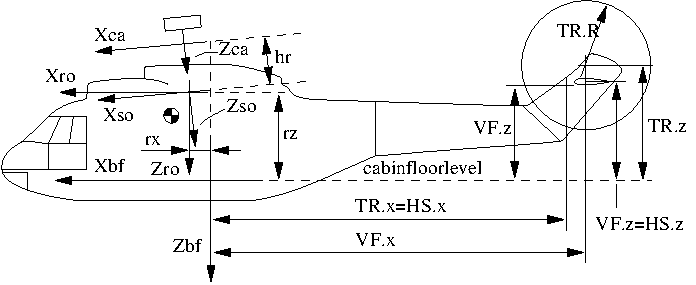
\includegraphics[width=0.7\textwidth]{./figs/chap_introduction/heli_sideview_pdf}
            \else
              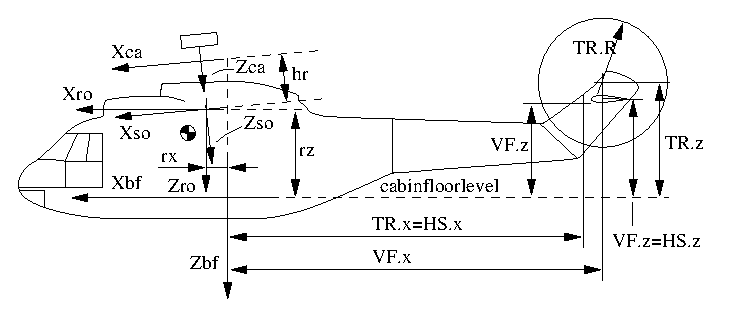
\includegraphics[width=0.7\textwidth]{./figs/chap_introduction/heli_sideview}
            \fi
            \caption[Short caption in the lof: schematic sideview of a helicopter]{Schematic sideview of a helicopter that is by now most likely too long to fit on one line.}
            \label{fig:sideview_reference_frames}
        \end{figure}
        %
%        \begin{figure}[!hbt]
%%             \tiny
%%             \scriptsize
%            \footnotesize
%            \psfrag{Xca}{$\mathsf{X_{hp}}$}
%            \psfrag{Zca}{$\mathsf{Z_{hp}}$}
%            \psfrag{Xro}{$\mathsf{X_{ro}}$}
%            \psfrag{Zro}{$\mathsf{Z_{ro}}$}
%            \psfrag{Xso}{$\mathsf{X_{so}}$}
%            \psfrag{Zso}{$\mathsf{Z_{so}}$}
%            \psfrag{Xbf}{$\mathsf{X_{bf}}$}
%            \psfrag{Zbf}{$\mathsf{Z_{bf}}$}
%            \psfrag{cabinfloorlevel}{$\mathsf{cabin floorlevel}$}
%            \psfrag{TR.R}{$\mathsf{R_{tr}}$}
%            \psfrag{TR.z}{$\mathsf{z_{tr}}$}
%            \psfrag{TR.x=HS.x}{$\mathsf{x_{vf}}$}
%            \psfrag{HS.z}{$\mathsf{z_{hs}}$}
%            \psfrag{VF.z=HS.z}{$\mathsf{z_{hs}}$}
%            \psfrag{VF.z}{$z_{vf}$}
%            \psfrag{VF.x}{$x_{tr} = x_{hs}$}
%            \psfrag{hr}{$h_{r}$}
%            \psfrag{rx}{$r_{x}$}
%            \psfrag{rz}{$r_{z}$}
%            \centering
%            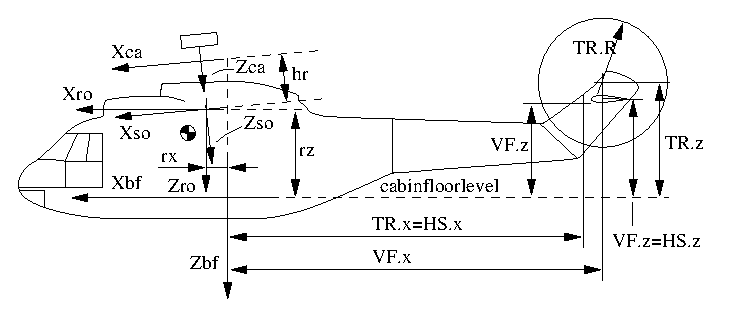
\includegraphics[width=0.7\textwidth]{./figs/chap_introduction/heli_sideview}
%            \caption{Schematic sideview of a helicopter (2)}
%            \label{fig:sideview_reference_frames_2}
%        \end{figure}
        %
        And a fancy figure to show you what is possible with graphics in \LaTeX, see Figure~\ref{fig:blade_geometry}.
        %
%        \begin{figure}[!htb]
%            \centering
%            \subfloat[Equal annuli segment distribution]{%
%                \begin{pspicture}(-0.25,-0.25)(13.125,1.2)
%                    % \psgrid[subgriddiv=1,griddots=10,gridlabels=7pt]
%                    \psdot*[dotsize=4pt](0,0)
%                    % quarter chord line
%                    \psline{-}(-0.25,0)(13.125,0)
%                    % vertical line through centre of rotation
%                    \psline{-}(0,-0.25)(0,0.25)
%                    % blade contours
%                    \pspolygon(3.0625,-0.2363)(13.125,-0.2363)(13.125,0.7088)(3.0625,0.7088)
%                    % blade segment sides
%                    \psline(5.0663,  -0.2363)( 5.0663,  0.7088)
%                    \psline(6.4775,  -0.2363)( 6.4775,  0.7088)
%                    \psline(7.6318,  -0.2363)( 7.6318,  0.7088)
%                    \psline(8.6333,  -0.2363)( 8.6333,  0.7088)
%                    \psline(9.5302,  -0.2363)( 9.5302,  0.7088)
%                    \psline(10.3495, -0.2363)( 10.3495, 0.7088)
%                    \psline(11.1085, -0.2363)( 11.1085, 0.7088)
%                    \psline(11.8190, -0.2363)( 11.8190, 0.7088)
%                    \psline(12.4891, -0.2363)( 12.4891, 0.7088)
%                    % control points
%                    \psdots*[dotsize=4pt](4.0644,  0.0)(5.7719,  0.0)(7.0546,  0.0)(8.1325,  0.0)(9.0817,  0.0)(9.9398,  0.0)(10.7290, 0.0)(11.4637, 0.0)(12.1540, 0.0)(12.8070, 0.0)
%                \end{pspicture}\label{subfig:equal_anulli_distribution}}\\
%            \subfloat[Constant width segment distribution]{%
%                \begin{pspicture}(-0.25,-0.25)(13.125,1.2)
%                    % \psgrid[subgriddiv=1,griddots=10,gridlabels=7pt]
%                    \psdot*[dotsize=4pt](0,0)
%                    % quarter chord line
%                    \psline{-}(-0.25,0)(13.125,0)
%                    % vertical line through centre of rotation
%                    \psline{-}(0,-0.25)(0,0.25)
%                    % blade contours
%                    \pspolygon(3.0625,-0.2363)(13.125,-0.2363)(13.125,0.7088)(3.0625,0.7088)
%                    % blade segment sides
%                    \psline(3.0625,  -0.2363)( 3.0625,  0.7088)
%                    \psline(4.0688,  -0.2363)( 4.0688,  0.7088)
%                    \psline(5.0750,  -0.2363)( 5.0750,  0.7088)
%                    \psline(6.0813,  -0.2363)( 6.0813,  0.7088)
%                    \psline(7.0875,  -0.2363)( 7.0875,  0.7088)
%                    \psline(8.0938,  -0.2363)( 8.0938, 0.7088)
%                    \psline(9.1000,  -0.2363)( 9.1000,  0.7088)
%                    \psline(10.1063, -0.2363)( 10.1063, 0.7088)
%                    \psline(11.1125, -0.2363)( 11.1125, 0.7088)
%                    \psline(12.1188, -0.2363)( 12.1188, 0.7088)
%                    \psline(13.1250, -0.2363)( 13.1250, 0.7088)
%                    % control points
%                    \psdots*[dotsize=4pt](3.5656,  0.00)(4.5719,  0.00)(5.5781,  0.00)(6.5844,  0.00)(7.5906,  0.00)(8.5969,  0.00)(9.6031,  0.00)(10.6094, 0.00)(11.6156, 0.00)(12.6219, 0.00)
%                \end{pspicture}\label{subfig:constant_width_distribution}}
%            \caption[Geometry for a helicopter main rotor blade]{Geometry and segment distributions for a helicopter main rotor blade with 10 segments} \label{fig:blade_geometry}
%        \end{figure}
        %
    \subsection{Alternatives}%
        %
        An alternative to saving figures as PostScript is saving them as PDF. Then, you have to use \emph{pdflatex} which skips the intermediate files. Please note that I will not provide support if you run into problems when you decide to do it this way.
        
        %
	%
    % Chapter 2 : Literature Review
    \chapter{Literature Review}
\label{ch:LiteratureReview}

%This is a detailed part of the proposal that rigorously reviews what work has been already carried out by other academics in this area while also benchmarking industry best practice. The researcher is trying to establish: 1) what research areas are relevant, and 2) what the current understanding is along with any opposing views. It is very nice to end with some sort of synthesis of the presented State-of-the-art to link explicitly to the work in the proposal, especially with regard to the following Section. This might even include a statement of what the author sees their work adding to the body of knowledge.

%%%%%%%%%%%%%%%%%%%%%%%%%%%%%%%%%%%%%%%%%%%%%%%%%%%%%%%%%%
\section{Current approaches}

\subsection{Momentum Theory}

\subsection{Single/Multiple Streamtube Model}

\subsection{Vortex Theory}

\subsubsection{Vortex Filament/Lifting Line Theory}

\subsubsection{Vortex particle Method}

\subsection{Full Navier-Stokes Model}

%%%%%%%%%%%%%%%%%%%%%%%%%%%%%%%%%%%%%%%%%%%%%%%%%%%%%%%%%%
\section{Purpose of further research}


%%%%%%%%%%%%%%%%%%%%%%%%%%%%%%%%%%%%%%%%%%%%%%%%%%%%%%%%%%
\section{Relevant research areas}

%\subsection{Domain decomposition methods}
%
%\subsubsection{Coupling techniques}
%
%\subsection{Simulation acceleration techniques}
%\section{Former Work}
%\label{sec:FormerWork}
%
%\subsection{Overview of the Work}
%\label{subsec:OverviewoftheWork}

%\section{Purpose of further research}

%%%%%%%%%%%%%%%%%%%%%%%%%%%%%%%%%%%%%%%%%%%%%%%%%%%%%%%%%%%%%%%%%%%%
%\nomenclature[ak]{$K$}{Kelvin (temperature)}
%\nomenclature[ar]{rpm}{Revolutions per minute (frequency)}
%\nomenclature[ac]{CO}{Carbon Monoxide}
%\nomenclature[ac]{CRM}{Chemical Reaction Modelling}
%\nomenclature[ah]{H2}{Molecular hydrogen}
%\nomenclature[ag]{GSP}{Gas Turbine Simulation Program (Software)}
%\nomenclature[rr]{$\rho$}{Density \nomunit{[$kg/{m^3}$]}}
%\nomenclature[sm]{$\dot{m}$}{Mass flow rate \nomunit{[$kg/s$]}}
%\nomenclature[ab]{bar}{Pressure}

%\nomenclature[rr]{$Re$}{Reynolds number \nomunit{[-]}}
%\nomenclature[rw]{$M$}{Mach number \nomunit{[-]}}
%\nomenclature[rw]{$\mu$}{Dynamic viscosity of air \nomunit{[$kg/{s \cdot m}$]}}
    %
    % Chapter 3: Literature review/Theory of Hybrid vortex methods
   	\chapter{Overview of Hybrid Vortex Methods}
%\label{ch:LiteratureReview}

% Comparison of hybrid vortex methods.
% choice of hybrid method. Example domain decomposion, coupling technique

\section{Theory}
% What is hybrid vortex method?
% What is the general idea behind the hybrid vortex method?
% What does it mean to couple particle solver and grid solver?
% What is the advantage?
% What is the drawback?

\section{Particle-Grid Coupling techniques}
% Multiple ways of coupling , VIC, domain decomposition technique
\subsection{Vortex in Cell method}

\subsection{Particle-Grid domain decomposition methods}

\section{Vortex diffusion methods}

\subsection{Random walk method}
\subsection{Core expansion method}
\subsection{Particle-Strength Exchange}
\subsection{Modified interpolation kernel for diffusion}

\section{Simulation acceleration techniques}

\subsection{Fast multi-pole Method}

\subsection{Parallel computation in GPU}

%\section{Former Work}
%\label{sec:FormerWork}
%
%\subsection{Overview of the Work}
%\label{subsec:OverviewoftheWork}

%\section{Purpose of further research}

%%%%%%%%%%%%%%%%%%%%%%%%%%%%%%%%%%%%%%%%%%%%%%%%%%%%%%%%%%%%%%%%%%%%
%\nomenclature[ak]{$K$}{Kelvin (temperature)}
%\nomenclature[ar]{rpm}{Revolutions per minute (frequency)}
%\nomenclature[ac]{CO}{Carbon Monoxide}
%\nomenclature[ac]{CRM}{Chemical Reaction Modelling}
%\nomenclature[ah]{H2}{Molecular hydrogen}
%\nomenclature[ag]{GSP}{Gas Turbine Simulation Program (Software)}
%\nomenclature[rr]{$\rho$}{Density \nomunit{[$kg/{m^3}$]}}
%\nomenclature[sm]{$\dot{m}$}{Mass flow rate \nomunit{[$kg/s$]}}
%\nomenclature[ab]{bar}{Pressure}

%\nomenclature[rr]{$Re$}{Reynolds number \nomunit{[-]}}
%\nomenclature[rw]{$M$}{Mach number \nomunit{[-]}}
%\nomenclature[rw]{$\mu$}{Dynamic viscosity of air \nomunit{[$kg/{s \cdot m}$]}}
   	%
   	% Chapter 4: Methodology of developing the hybrid vortex method
    \chapter{Development of the Hybrid Vortex Method for 2D VAWT}
%\label{ch:LiteratureReview}

% Comparison of hybrid vortex methods.
% choice of hybrid method. Example domain decomposion, coupling technique

\section{Methodology}
% What is hybrid vortex method?
% What is the general idea behind the hybrid vortex method?
% What does it mean to couple particle solver and grid solver?
% What is the advantage?
% What is the drawback?

\section{Vortex Method}
% All the info on the development of vortex method
% What approach are you using?
% G. Daenick, G. Winckelmans method

%\documentclass[10pt,a4paper,twocolumn]{article}
%\documentclass[10pt,a4paper]{article}

% Extra packages
%\usepackage{fullpage}
%\usepackage[utf8]{inputenc}
%\usepackage{amsmath}
%\usepackage{amsfonts}
%\usepackage{amssymb}
%\usepackage{graphicx}
%\usepackage{hyperref}

%\usepackage{graphicx}
%\usepackage{caption}
%\usepackage{subcaption}

% Document description
\title{Convergence of modified interpolation kernel for treating diffusion}
\author{Lento Manickathan, 1544101.\\Aerodynamics and Wind energy}

% Begin of main body
%\begin{document}

% Show title
%\maketitle

% Main content

\section{Introduction to modified interpolation kernel for treating diffusion}
The diffusion method that is applied here has been proposed by Shankar and Van Dommelen \cite{Shankar1996} and the modified ${{{\rm{M'}}}_4}$ interpolation kernel has been derived by Ghoniem and Wee \cite{Wee2006} and was also applied by Speck \cite{Speck2011}. The diffusion is simulated by the modified interpolation kernel during the remeshing process. During remeshing, the heat equation is satisfied by transferring the correct fraction of circulation to produce the proper amount of diffusion. The ${{{\rm{M'}}}_4}$ kernel was modified to treat the diffusion and is given by: 

\begin{equation}
{{{\rm{M'}}}_4}\left( {\xi ,c} \right) =
  \begin{cases}
   {1 - \frac{{5{\xi ^2}}}{2} + \frac{{3{{\left| \xi  \right|}^3}}}{2} - {c^2}\left( {2 - 9{\xi ^2} + 6{{\left| \xi  \right|}^3}} \right)} & {\left| \xi \right|} < 1, \\
   \frac{1}{2}{\left( {2 - \left| \xi  \right|} \right)^2}\left( {1 - \left| \xi  \right|} \right) - {c^2}{\left( {2 - \left| \xi  \right|} \right)^2}\left( {1 - 2\left| \xi  \right|} \right) & 1 \le {\left| \xi \right|} < 2,\\
   0 & 2 \le \left| \xi \right|,
  \end{cases}
\label{eq:modInterpKernel}
\end{equation}

where 

\begin{equation}
c = \frac{\sqrt{\nu \Delta t_d}}{\Delta x},
\label{eq:c2}
\end{equation}

and corresponds to the transfer quantity for diffusion. The $\nu$ denotes the viscosity of the fluid, $t_d$ is the diffusion time step and $\Delta x$ is the blob spacing. When $c \rightarrow 0$, the interpolation kernel turns to the classical non-diffusion kernel.  This modified interpolation kernel conserves the circulation of each vortex and also satisfies the conservation of linear and angular momentum of the vorticies.\\

The vortex method employs the viscous splitting procedure, where the vortex blobs are convected first and is then diffused through the remeshing process using the modified interpolation kernel. The advantage of this methodology is that the convection process is not constrained by the CFL condition. So, the convection time step size can be different than from the diffusion time step size and the diffusion time step size is a multiple of the convection time step size depending on the redistribution frequency $f_{redist}$. Therefore, the constrained that is imposed on the redistribution frequency is the stability bounds of the modified interpolation kernel. Analyzing the amplification factor and the phase error of the modified interpolation kernel in the Fourier space requires that the $c^2$ should be as follows:


\begin{equation}
\frac{1}{6} \le c^2 \le \frac{1}{2}.
\label{eq:c2stability}
\end{equation}

This will ensure the stability of the problem and will suppress any spurious oscillations and ensure that it is a non-negative interpolation kernel with non-negative redistribution fractions.

\section{Errors in Blob Initialization}
To verify the accuracy of the diffusion process, the error of the discrete solution was compared against the analytical solution of the Lamb-Oseen vortex where the vorticity field

\begin{equation}
\omega\left(x,t\right) = \frac{\Gamma_o}{4\pi \nu t} \exp \left(-\frac{r^2}{4 \nu t} \right),
\label{eq:LambOseen}
\end{equation}

was used as the analytical solution for a given viscosity $\nu$ at a given time $t$ with a unit circulation $\Gamma_o$. In order to quantify the error generated during discretization, the discrete $L^2$-norm error was calculated as 

\begin{equation}
{\left\| {{\omega ^{{\rm{exact}}}} - {\omega ^{{\rm{discrete}}}}} \right\|_2} = {\left( {\sum\limits_i {{{\left| {{\omega ^{{\rm{exact}}}}({{\bf{x}}_i}) - {\omega ^{{\rm{discrete}}}}({{\bf{x}}_i})} \right|}^2}\Delta x\Delta y} } \right)^{\frac{1}{2}}},
\label{eq:L2normEq}
\end{equation} 	

and the discrete maximum relative error in vorticity was evaluated as follows:

\begin{equation}
{\left\| {{\omega ^{{\rm{exact}}}} - {\omega ^{{\rm{discrete}}}}} \right\|_\infty } = \frac{{\max \left\{ {\left| {{\omega ^{{\rm{exact}}}}({{\bf{x}}_i}) - {\omega ^{{\rm{discrete}}}}({{\bf{x}}_i})} \right|:i \in {\mathcal{S}}} \right\}}}{{\max \left\{ {\left| {{\omega ^{{\rm{exact}}}}({{\bf{x}}_i})} \right|:i \in {\mathcal{S}}} \right\}}}.
\label{eq:maxRelEq}
\end{equation}

During the initial discretization, it was seen that in order to obtain the correct vorticity field, you need to take in account of the numerical diffusion. As Barba had shown in \cite{Barba2004a}, in order to properly account for the diffusion effect when discretization with gaussian blobs (with $k=2$), a time-shift correction equivalent to shifting the initial time by $\sigma^2/2\nu$ needs to be applied. This follows directly from the discretization of the general solution of the heat equation with these gaussian cores. With this proper time-shifting, you can ensure the accurate initialization of the Lamb-Oseen vortex for the error evaluations. \\

An alternate method of taking account for the gaussian approximation is the Beale's iterative method for circulation processing. The concept is based on iteratively improving the circulation values of the gaussian blobs so that it gives a better approximation of the local vorticity that the blobs are trying to represent. The downside to this processing is that the influence matrix for the calculation is $\mathcal{O}(N^2)$ and requires large computational resources.

\section{Importance of initial conditions}



\begin{itemize}
\item Comparing $\nu=0.01$ and $\nu=0.0005$ with various starting times. Show the growth in error. 
\item Compare various correction methods for initial discretization. Beale vs. time-shifting
\end{itemize}

\section{Convergence of the vortex method with diffusion}
The discretization errors of the vortex method was evaluated to check for the convergence of its error to the exact solution. If the modified interpolation kernel was accurately implemented into the vortex method, the spatial and the temporal discretization error of the vortex method should converge as you refine the parameters. When checking for discretization error a given parameter, all the other parameters was kept constant and at a very high resolution. This ensured that the significant error emerges from the discretization of the chosen parameter. For the initial investigations, this meant that the $c^2$ parameter of the kernel diffusion term was also varying dependent on the discretization parameter. This could indirect influence on the convergence rate, as diffusion term was varying for each discrete value. So, a second investigation was done, where the $c^2$ parameters was kept constant by varying the appropriate values.

To ensure that other numerical error does not dominate and the consistency of the simulations, all the variables were carefully chosen and are tabulated in table \ref{tab:refinementParameters}.\\

\begin{table}[hbt]
\centering
	\begin{tabular}{|l|r|}
	\hline \textbf{Parameters} 					& \textbf{Value} \\
	\hline Domain $\Omega$ 						& $[-2, 2]^2$ \\
	Overlap ratio $\Delta h/\sigma$  	& 0.5  \\ 
	Viscous time scale $\tau$ 			& 0.0200 to 0.0250 \\
	Time step scheme 					& RK4 \\
	Vortex viscosity $\nu$ 				& [0.01, 0.0005] \\
	Vortex Circulation Strength $\Gamma$ & $2 \pi$ \\
	Vortex Reynolds Number Re 			& [50, 2000] \\
	Vortex Reynolds Number Re 			& [50, 2000] \\
	Kernel diffusion parameter $c^2$		& $1/6$, $1/4$, $1/2$ \\
	Redistribution frequency $f_{redist}$& 1 \\
	Population control $\Gamma_{min}$ 	& \texttt{eps} $ = 2.2e$\textrm{-}$16$\\
	Population control frequency $f_{pc}$& 1 \\
	\hline 
	\end{tabular} 
\caption{Refinement study parameters}
\label{tab:refinementParameters}
\end{table}


\subsection{Blob density refinement study}
In order to investigate the convergence of the error and as the spatial discretization is refined, a blob density refinement study was undertaken. By increasing the number of blob cores to represent the given vortex, the discrete approximation of the vortex should converge to the exact solution. In order words, as the spatial discretization $\Delta y$ and $\Delta y$ is reduced, the error should converge.

During the investigation of the blob density (number of particles) refinement, the time step was maintained at a minimum to reduce its error, $\delta T = 0.05$. Investigation was done for two viscous cases, as shown in table \ref{tab:refinementParameters}. This results in time step parameters as shown in table \ref{tab:spatialRefinementParameters}.

\begin{table}[hbt]
\centering
	\begin{tabular}{|l|r|r|}
	\hline \textbf{Parameters} 	& \textbf{$\nu = 0.01$} & \textbf{$\nu = 0.0005$}\\
	\hline Start time $\tau/\nu$    & 2 & 40 \\				
	Stop time  $\tau/\nu$ 	& 2.5 & 50 \\
	Number of steps 			& 10 & 200 \\
	Number of blobs 			& [73, 86, 98, 108, 118, 126] & [327, 386, 438, 484, 527, 566]\\
	\hline
	\end{tabular}
\caption{Blob density refinement study parameters}
\label{tab:spatialRefinementParameters}	
\end{table}

The results of the spatial refinement is shown in figure \ref{fig:wErrorVSdx_varyingC2}. 

\begin{figure}[!tbhp]
\centering
	\begin{subfigure}{0.48\textwidth}
		\centering
		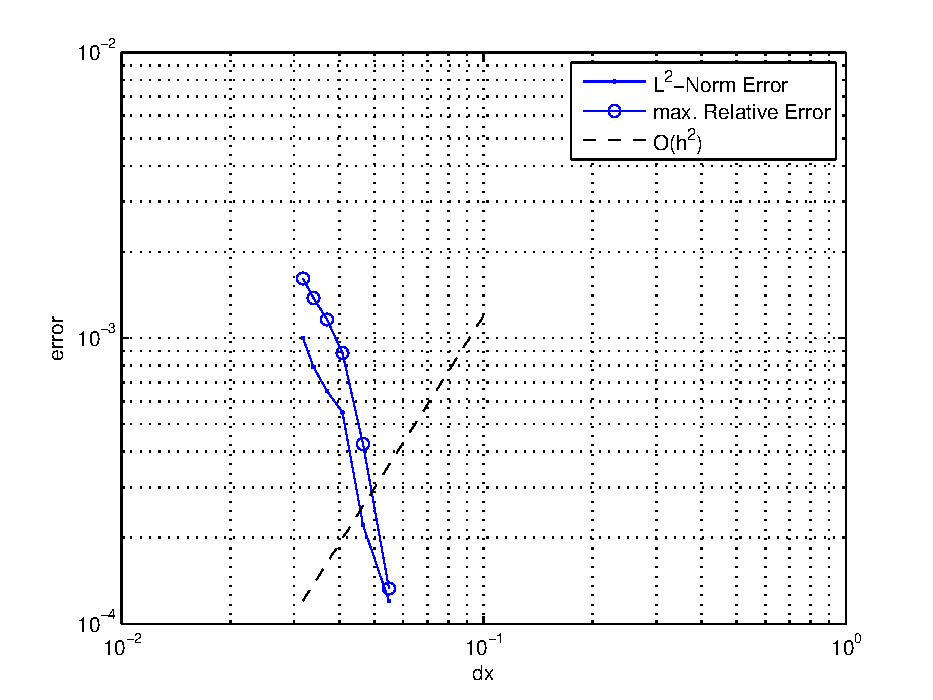
\includegraphics[width=\textwidth]{./figures/wErrorVSdx_nu001_c2vary.pdf}	
		\caption{$\nu=0.01$}
	\end{subfigure}
	\begin{subfigure}{0.48\textwidth}
		\centering
		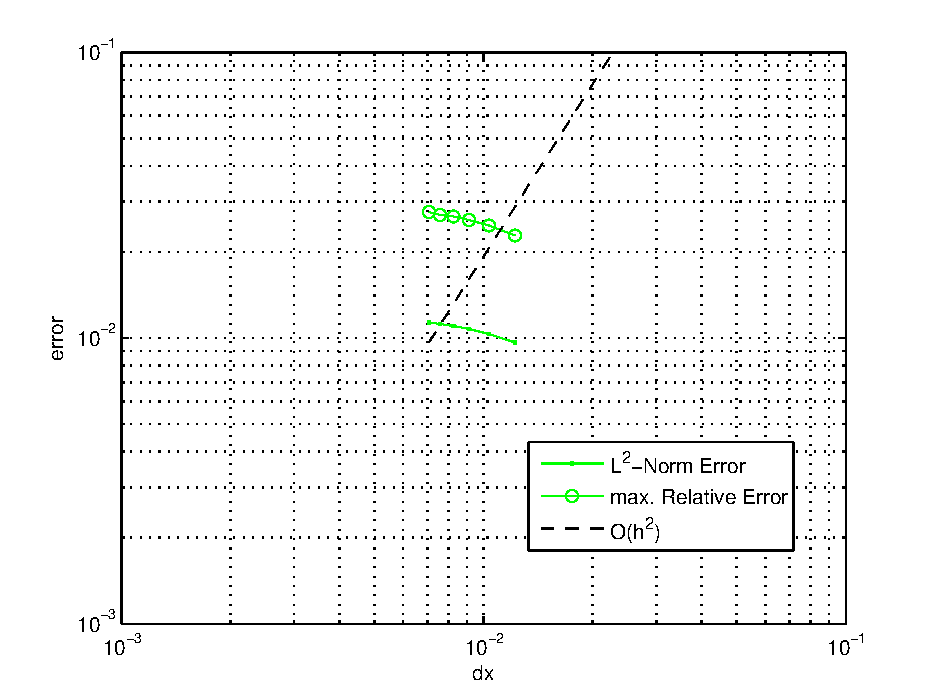
\includegraphics[width=\textwidth]{./figures/wErrorVSdx_nu00005_c2vary.pdf}	
		\caption{$\nu=0.0005$}
	\end{subfigure}
\caption{Spatial refinement with a varying $c^2$}
\label{fig:wErrorVSdx_varyingC2}
\end{figure}

It is evident that the order of convergence does not match the predicted one. This is because of the one key parameter, the kernel diffusion parameter $c^2$. We assume that as the number of particles (i.e blob density) increases, the spatial discretization $\Delta h$ reduces thereby resolving the Lamb-Oseen vortex to greater detail. However, from equation \ref{eq:c2} we see that if viscosity $nu$ and time step $\Delta T$ is constant then $\Delta $ is inverse proportional to kernel diffusion parameter $c^2$. This means that the $c^2$ parameter is increasing and has a direct influence of the damping of the numerical oscillations. Therefore, as the $c^2$ increase, the growth in error might be more dominant and could have an effect on the spatial refinement study.\\

So, to have a proper comparison, the spatial refinement study was done with keeping the $c^2$ parameter constant, figure \ref{fig:wErrorVSdx_constantC2}.

\begin{figure}[!tbhp]
\centering
	\begin{subfigure}{0.48\textwidth}
		\centering
		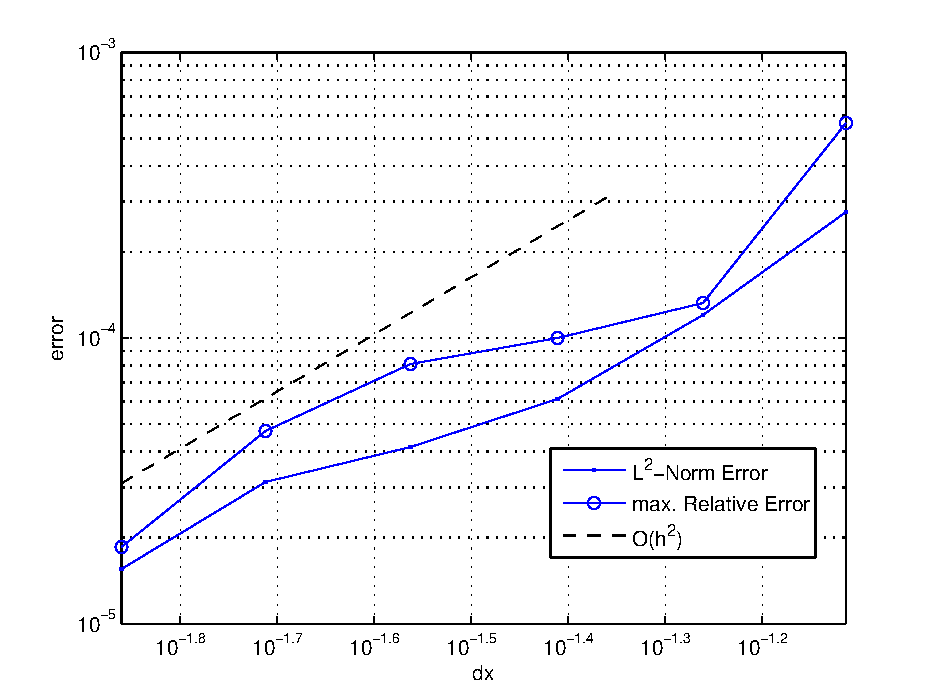
\includegraphics[width=\textwidth]{./figures/wErrorVSdx_nu0p01_constantc2.pdf}	
		\caption{$\nu=0.01$}
	\end{subfigure}
	\begin{subfigure}{0.48\textwidth}
		\centering
		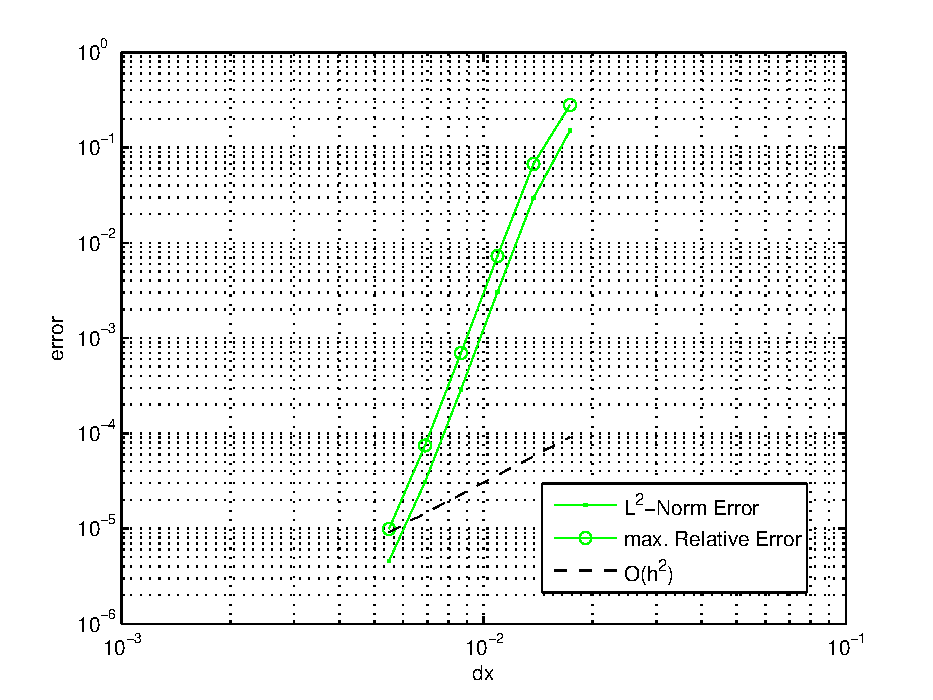
\includegraphics[width=\textwidth]{./figures/wErrorVSdx_nu0p0005_constantc2.pdf}	
		\caption{$\nu=0.0005$}
	\end{subfigure}
\caption{Spatial refinement with a constant $c^2=1/6$}
\label{fig:wErrorVSdx_constantC2}
\end{figure}

Now we can see that the error converges as you reduced the blob mesh size. This is the correct trend that we are looking for.

\subsection{Spatial refinement for various kernel diffusion parameter}

\begin{figure}[!tbhp]
\centering
	\begin{subfigure}{0.48\textwidth}
		\centering
		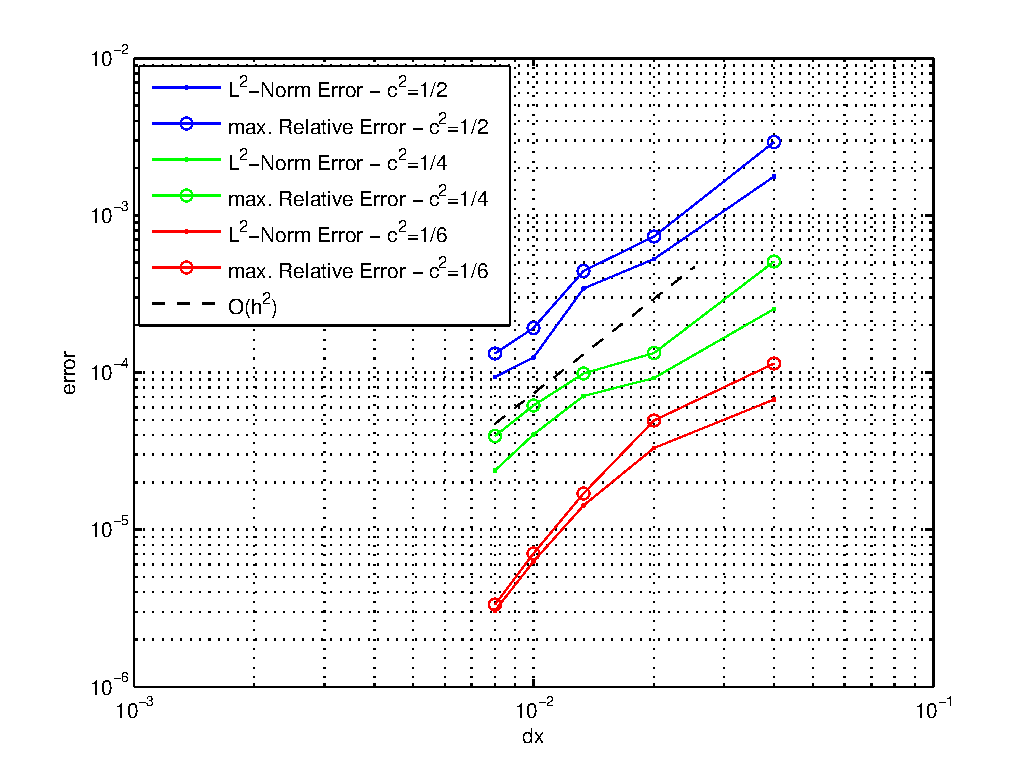
\includegraphics[width=\textwidth]{./figures/wErrorVSdx_nu0p01_variousC2.pdf}	
		\caption{$\nu=0.01$}
	\end{subfigure}
	\begin{subfigure}{0.48\textwidth}
		\centering
		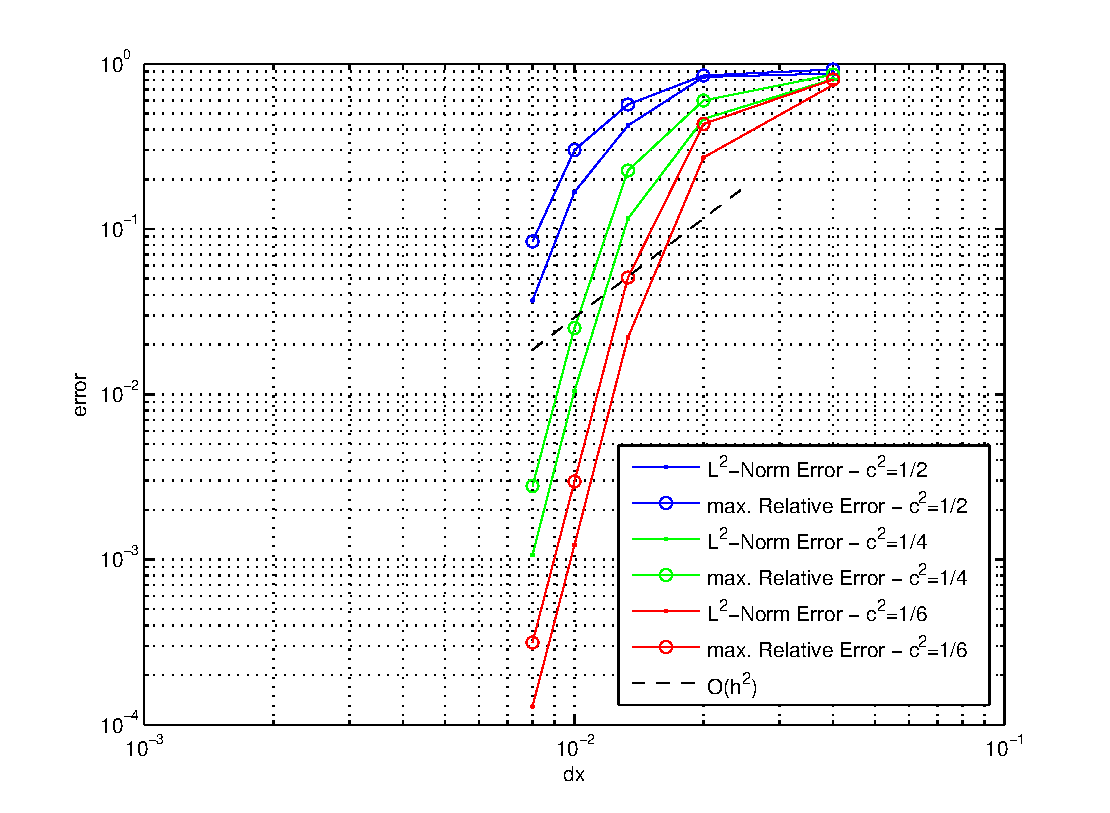
\includegraphics[width=\textwidth]{./figures/wErrorVSdx_nu0p0005_variousC2.pdf}	
		\caption{$\nu=0.0005$}
	\end{subfigure}
\caption{Spatial refinment for various $c^2$ parameters, $c^2 = [\frac{1}{6}, \frac{1}{4}, \frac{1}{2}]$}
\label{fig:wErrorVSdx_variousC2}
\end{figure}



\subsection{Time Step refinement study}

\begin{figure}[!tbhp]
\centering
	\begin{subfigure}{0.48\textwidth}
		\centering
		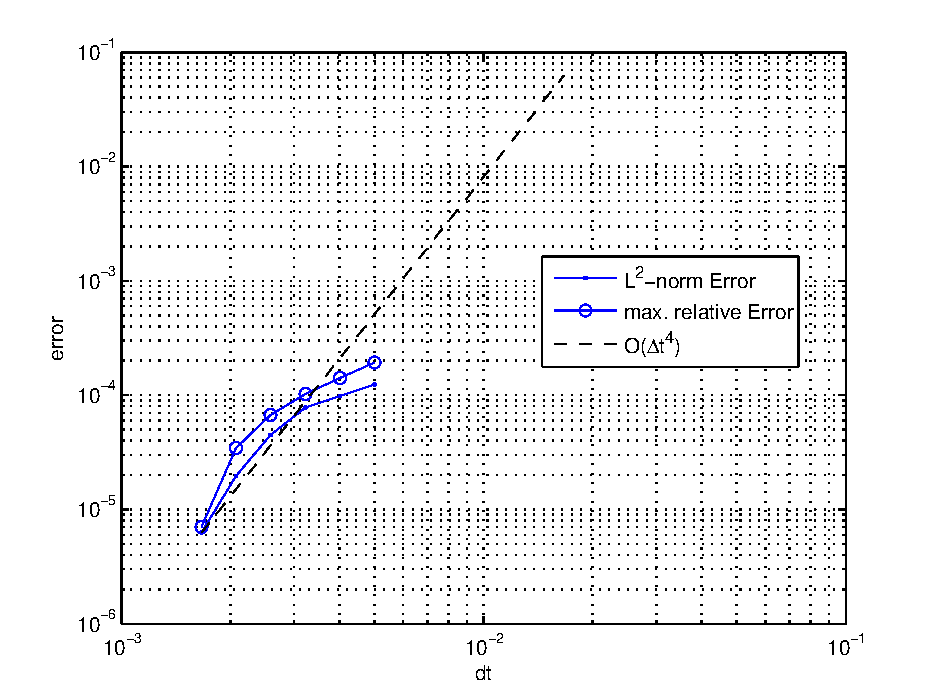
\includegraphics[width=\textwidth]{./figures/wErrorVSdt_nu0p01_varyingC2.pdf}	
		\caption{$\nu=0.01$}
	\end{subfigure}
	\begin{subfigure}{0.48\textwidth}
		\centering
		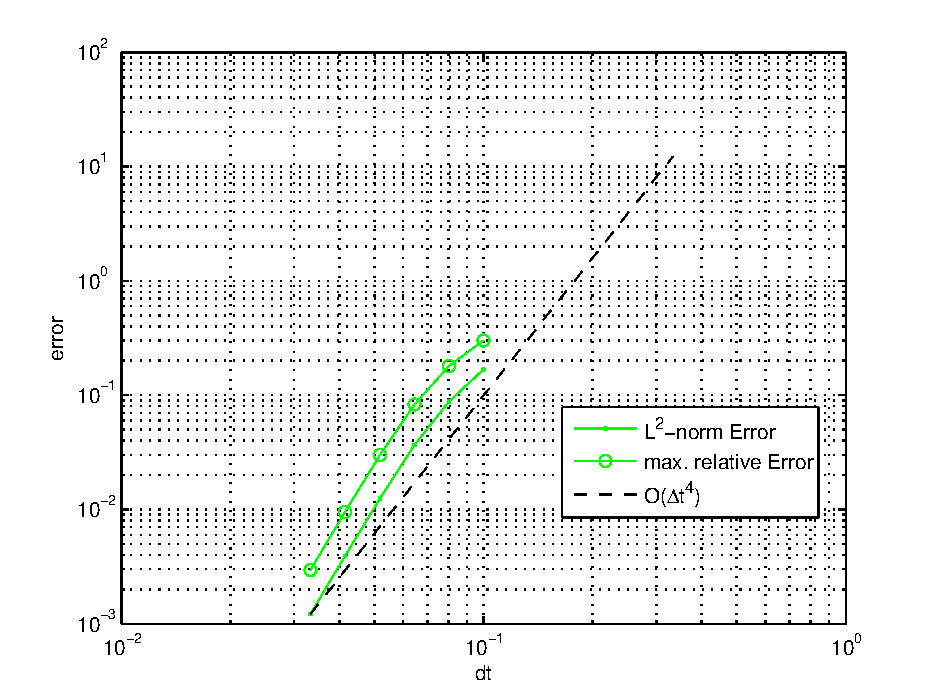
\includegraphics[width=\textwidth]{./figures/wErrorVSdt_nu0p0005_varyingC2.pdf}	
		\caption{$\nu=0.0005$}
	\end{subfigure}
\caption{Time Step refinement with a varying $c^2$}
\label{fig:wErrorVSdt_varyingC2}
\end{figure}





% End of main body
\newpage

% Bibliography
%\bibliographystyle{plain}
%\bibliography{../../Literature/library}

% End of document
%\end{document}

\subsection{Blob Discretization}
% Particle initialization
% info on cut-off function
% what are the governing variables? Overlap ratio, grid size, 

\subsubsection{Error analysis of discretization}
% importance of time-shift correction when comparing with Lamb-oseen
% overlap ratio vs. L2-norm and max.relative error
% number of particles/ deltaH vs. L2-norm and max.relative error

\subsection{Vortex blob convection}
% Info on time-stepping scheme
% source of error during convection = lagrangian distortion from fluid strain
% importance of population control

\subsubsection{Remeshing for lagrangian grid distortion}
% show with and without remeshing figure.
% investigate on remeshing frequence -> treatment of vortex diffusion

\subsubsection{Error of time-Stepping}
% Time-step vs. L2-norm and max.relative error
% Show the convergence of time-step scheme

\subsection{Treatment of vortex diffusion with remeshing}
% refer to Daehyun Wee, Ahmed F. Ghoniem 2006
% Brief overview of other methods
% motivation of the choice of modified interpolation kernel, diffusion through remeshing


\subsubsection{Modified interpolation kernel}
% Equation for modified interpolation kernel, 
% M4 kernel
% Stability condition, And also conclusion to c2 parameter. the range for the value 1/6<= c2 <=1/2

\subsubsection{Convergence of modified interpolation kernel}
% Comparison with L.Barba, Phd.Thesis
% evolution of error in vorticity of Lamb-oseen.
% 

%%%%%%%%
\subsection{Treatment of geometry in fluid}

\subsubsection{Vortex sheet for inviscid boundary condition}
% using vortex sheet to solve boundary integral equation
% refer to using RBF kernels as a mesh-less solution, recommendations.

\subsubsection{Convergence of panel method}


%%%%%%%
\section{Coupling grid to particle solver}

\subsection{Coupling algorithm and modified overlap region}


\section{Moving boundaries}
\subsection{Modification to grid solver}
\subsection{Modification to vortex method}


%\section{Former Work}
%\label{sec:FormerWork}
%
%\subsection{Overview of the Work}
%\label{subsec:OverviewoftheWork}

%\section{Purpose of further research}

%%%%%%%%%%%%%%%%%%%%%%%%%%%%%%%%%%%%%%%%%%%%%%%%%%%%%%%%%%%%%%%%%%%%
%\nomenclature[ak]{$K$}{Kelvin (temperature)}
%\nomenclature[ar]{rpm}{Revolutions per minute (frequency)}
%\nomenclature[ac]{CO}{Carbon Monoxide}
%\nomenclature[ac]{CRM}{Chemical Reaction Modelling}
%\nomenclature[ah]{H2}{Molecular hydrogen}
%\nomenclature[ag]{GSP}{Gas Turbine Simulation Program (Software)}
%\nomenclature[rr]{$\rho$}{Density \nomunit{[$kg/{m^3}$]}}
%\nomenclature[sm]{$\dot{m}$}{Mass flow rate \nomunit{[$kg/s$]}}
%\nomenclature[ab]{bar}{Pressure}

%\nomenclature[rr]{$Re$}{Reynolds number \nomunit{[-]}}
%\nomenclature[rw]{$M$}{Mach number \nomunit{[-]}}
%\nomenclature[rw]{$\mu$}{Dynamic viscosity of air \nomunit{[$kg/{s \cdot m}$]}}
   	%
   	% Chapter 5: Validation of Hybrid Vortex Method
   	\chapter{Validation of the Hybrid Vortex Method}
%\label{ch:LiteratureReview}

% Comparison of hybrid vortex methods.
% choice of hybrid method. Example domain decomposion, coupling technique

\section{Fixed boundary}

\subsection{Dipole-wall interaction}

\subsection{Impulsively started flow past cylinder}

\section{Cascading airfoil}

\section{Moving boundary}

\section{Pitching airfoil}

%\section{Former Work}
%\label{sec:FormerWork}
%
%\subsection{Overview of the Work}
%\label{subsec:OverviewoftheWork}

%\section{Purpose of further research}

%%%%%%%%%%%%%%%%%%%%%%%%%%%%%%%%%%%%%%%%%%%%%%%%%%%%%%%%%%%%%%%%%%%%
%\nomenclature[ak]{$K$}{Kelvin (temperature)}
%\nomenclature[ar]{rpm}{Revolutions per minute (frequency)}
%\nomenclature[ac]{CO}{Carbon Monoxide}
%\nomenclature[ac]{CRM}{Chemical Reaction Modelling}
%\nomenclature[ah]{H2}{Molecular hydrogen}
%\nomenclature[ag]{GSP}{Gas Turbine Simulation Program (Software)}
%\nomenclature[rr]{$\rho$}{Density \nomunit{[$kg/{m^3}$]}}
%\nomenclature[sm]{$\dot{m}$}{Mass flow rate \nomunit{[$kg/s$]}}
%\nomenclature[ab]{bar}{Pressure}

%\nomenclature[rr]{$Re$}{Reynolds number \nomunit{[-]}}
%\nomenclature[rw]{$M$}{Mach number \nomunit{[-]}}
%\nomenclature[rw]{$\mu$}{Dynamic viscosity of air \nomunit{[$kg/{s \cdot m}$]}}
	%
	% Chapter 6: Applications of Hybrid vortex method
	\chapter{Application of the Hybrid Vortex Method}
%\label{ch:LiteratureReview}

% Comparison of hybrid vortex methods.
% choice of hybrid method. Example domain decomposion, coupling technique

\section{Application of Hybrid Vortex method for a 2D VAWT}

\subsection{Reference setup}

\subsection{Instantaneous flow-field}

\subsection{Time averaged flow-field}

\subsection{Near-wake}

\subsubsection{Dynamic Stall of the airfoil}

\subsection{Far-wake}

\subsubsection{Blade-wake interaction}

\section{Feasibility of Hybrid Vortex method for compressor cascade}

\subsection{Assumptions and approximations}

\subsection{Advantages of hybrid vortex method}

\subsection{Limitation of using hybrid vortex method}

\subsection{Proposed solution}



%\section{Former Work}
%\label{sec:FormerWork}
%
%\subsection{Overview of the Work}
%\label{subsec:OverviewoftheWork}

%\section{Purpose of further research}

%%%%%%%%%%%%%%%%%%%%%%%%%%%%%%%%%%%%%%%%%%%%%%%%%%%%%%%%%%%%%%%%%%%%
%\nomenclature[ak]{$K$}{Kelvin (temperature)}
%\nomenclature[ar]{rpm}{Revolutions per minute (frequency)}
%\nomenclature[ac]{CO}{Carbon Monoxide}
%\nomenclature[ac]{CRM}{Chemical Reaction Modelling}
%\nomenclature[ah]{H2}{Molecular hydrogen}
%\nomenclature[ag]{GSP}{Gas Turbine Simulation Program (Software)}
%\nomenclature[rr]{$\rho$}{Density \nomunit{[$kg/{m^3}$]}}
%\nomenclature[sm]{$\dot{m}$}{Mass flow rate \nomunit{[$kg/s$]}}
%\nomenclature[ab]{bar}{Pressure}

%\nomenclature[rr]{$Re$}{Reynolds number \nomunit{[-]}}
%\nomenclature[rw]{$M$}{Mach number \nomunit{[-]}}
%\nomenclature[rw]{$\mu$}{Dynamic viscosity of air \nomunit{[$kg/{s \cdot m}$]}}
    %
    % Chapter 7: 
	\chapter{Conclusion and Recommendation}
\label{ch:ConclusionandRecommendation}

\section{Conclusion}

\subsection{Feasibility of hybrid vortex method for compressor cascade}

\section{Recommendations}

\subsection{RBF kernel representation of boundary}

\subsection{Recommended numerical simulation for compressor cascade}
    
    %
    % Bibliography
    \printbib{biblio}%
    %
    \appendix%
    %
    % and some appendices here
    \chapter{Mathematical Model}\label{app:math_model_main_rotor}%
    %
    \section{Introduction}%
        %
        This appendix contains the math model of the thesis. It looks as follows:
        %
        \begin{equation}
            c = \sqrt{a^2+b^2}
        \end{equation}
        %
        
        
        
        
        
        
%
    %
    %
\backmatter%
    %
    % index file here (not needed for a MSc thesis)
    %
\end{document}
